% !TeX program = xelatex
% UTF-8. Compile twice: xelatex manuscript.tex
\documentclass[UTF8,a4paper,11pt,fontset=fandol]{ctexart}
\usepackage[margin=25mm]{geometry}
\usepackage{amsmath,amssymb,booktabs,graphicx}
\usepackage[hidelinks,unicode]{hyperref}
\setlength{\emergencystretch}{2em}
\ctexset{section={format=\Large\bfseries},subsection={format=\large\bfseries}}
\title{窄栅栏网格的燃烧数}
\author{}
\date{}
\begin{document}
\maketitle

\begin{abstract}
设 $G_{m,n}$ 为 $m$ 行、$n$ 列的笛卡尔网格。对于 $m=\lfloor c\sqrt{n}\rfloor$ 且 $0<c\le 2/\sqrt{5}$ 的情形，我们构造一个离散菱形覆盖，使燃烧数达到 Bonato 等人所得边界下界的首项，并将余项控制为 $O(1)$。构造的核心是将相邻两个大菱形的中心错开一行，用一对半径互补的小菱形恰好填满两侧的整数缺口。对于 $c=1$，同一构造还给出一个改进的上界。
\end{abstract}

\section{模型与结论}

记 $G_{m,n}=P_m\square P_n$。顶点为 $(x,y)$，其中 $0\le x<n$、$0\le y<m$；相邻点的曼哈顿距离为 $1$。每轮从此前未燃的顶点中选一个点燃，此前已经燃烧的顶点同时把火传给邻点。最少轮数记为 $b(m,n)$。水平和竖直坐标均从 $0$ 起算，$y=0$ 表示下边界。下文的列数、行数均包含两个端点。

\textbf{定理 1.} 固定 $0<c\le 2/\sqrt{5}$。当 $n\to\infty$ 时，

\[
b(\lfloor c\sqrt{n}\rfloor,n)
=\left(\frac c2+\sqrt{1-\frac{c^2}{4}}\right)\sqrt{n}+O_c(1).
\]

\textbf{定理 2.} 记 $\beta=(3+\sqrt{261})/14$。对一切充分大的 $n$，

\[
b(\lfloor\sqrt{n}\rfloor,n)\le \lceil\beta\sqrt{n}\rceil+2.
\]

Bonato、English、Kay 和 Moghbel 在文献 [1，第 4 节] 提出确定栅栏网格燃烧数首项常数的问题。他们的边界计数给出定理 1 中的下界系数。对于 $c=1$，他们给出的下、上界系数分别为 $(1+\sqrt{3})/2\approx1.366025$ 和 $(2+\sqrt{15})/4\approx1.468246$。定理 2 将后者降至 $\beta\approx1.368250$；此处的确切首项常数仍待确定。本文不声称下界系数本身为新结果；贡献在于给出一个显式覆盖构造，使上界在 $0<c\le 2/\sqrt{5}$ 内达到该下界的首项，并在 $c=1$ 时将显式上界系数从 $1.468246$ 降至 $1.368250$。此外，对一切充分大的 $n$，定理 2 也给出 $b(\lfloor\sqrt{n}\rfloor,n)\le \beta\sqrt{n}+O(1)$。

\textbf{覆盖表述.} 在 $k$ 轮结束时，第 $t$ 轮的火能到达以其火源为中心、半径 $k-t$ 的闭球。反过来，若半径 $k-1,k-2,\ldots,0$ 的球各用一次即可盖住网格，便可按此顺序点火：若第 $t$ 个预定中心已燃，它到第 $k$ 轮仍可把火传遍其预定球，此轮可改点任一此前未燃的顶点。若已全燃则提前结束。因此，寻求 $b(m,n)\le k$ 等价于寻求这样的覆盖。

\section{奇数行网格的有限构造}

取正整数 $p,h,k$ 满足 $p\le h\le 2p$、$k\ge 3p+1$。先在无限长的格点条带 $\mathbb{Z}\times\{0,\ldots,2h\}$ 内布置火源。令

\[
d=h-p,\qquad B=k-2p,\qquad
r_i=k-1-i,\qquad a_i=d+\min(i,p)
\quad(0\le i<B).
\]

第 $i$ 个大球半径为 $r_i$，中心为 $(x_i,a_i)$，取 $x_0=0$。因 $B\ge p+1$，前 $p$ 个接缝都存在；最后一个大球的中心高度为 $h$。对 $0\le i<B-1$，定义

\begin{equation}\label{eq:spacing}
x_{i+1}-x_i=
\begin{cases}
r_i+r_{i+1}-2d+1, & 0\le i<p,\\
r_i+r_{i+1}-2h+1, & p\le i<B-1.
\end{cases}
\end{equation}

对每个 $0\le i<p$，另置下、上两个小球，中心和半径依次为

\begin{equation}\label{eq:small}
\begin{aligned}
&(z_i^{-},0),  &z_i^{-}&=x_i+r_i-d+1, &\text{半径}&\quad i,\\
&(z_i^{+},2h), &z_i^{+}&=x_i+r_i-d,   &\text{半径}&\quad s_i=2p-1-i.
\end{aligned}
\end{equation}

两组小半径分别用尽 $0,\ldots,p-1$ 和 $p,\ldots,2p-1$；大半径用尽 $2p,\ldots,k-1$。恰好每个半径用一次。

\subsection{逐行补缝}

第 $i$ 个大球在整数行 $y$ 的截面是以 $x_i$ 为中心、半宽 $u_i(y)=r_i-|y-a_i|$ 的闭整数区间。这里 $u_i(y)\ge0$：若 $i\le p$，到较远边界的距离为 $2h-a_i=h+p-i\le k-1-i$；若 $i\ge p$，该距离为 $h\le2p\le r_i$。因此每个大球覆盖自己的整条中心列。

对相邻的两个大球，令 $E=x_i+u_i(y)+1$、$F=x_{i+1}-u_{i+1}(y)-1$。缺口为 $[E,F]\cap\mathbb{Z}$；当 $E>F$ 时它为空。对于 $i<p$ 有 $a_{i+1}=a_i+1$。代入式 \eqref{eq:spacing}，得到两组精确端点。

当 $y\le a_i$ 时，$u_i=r_i-a_i+y$，$u_{i+1}=r_{i+1}-a_i-1+y$，故

\begin{equation}\label{eq:lower-gap}
(E,F)=\bigl(z_i^{-}-(i-y),\ z_i^{-}+(i-y)\bigr).
\end{equation}

若 $y\le i$，这恰是下方半径 $i$ 的球在该行的截面；若 $i<y\le a_i$，则缺口为空。

当 $y\ge a_i+1$ 时，$u_i=r_i-y+a_i$，$u_{i+1}=r_{i+1}-y+a_i+1$。记 $q_i(y)=s_i-(2h-y)=y-2d-i-1$，则

\begin{equation}\label{eq:upper-gap}
(E,F)=\bigl(z_i^{+}-q_i(y),\ z_i^{+}+q_i(y)\bigr).
\end{equation}

若 $q_i(y)\ge0$，这恰是上方半径 $s_i$ 的球在该行的截面；否则缺口为空。相邻整数 $a_i,a_i+1$ 之间没有其他整数行，故式 \eqref{eq:lower-gap}、\eqref{eq:upper-gap} 穷尽所有情形。特别地，两个小球的横坐标相差一列。

若 $p\le i<B-1$，相邻大球均在中线。由 $u_j(y)\ge r_j-h$ 和式 \eqref{eq:spacing}，有 $x_{i+1}-u_{i+1}(y)\le x_i+u_i(y)+1$，两个区间相交或相邻。这证明了从第一条中心列到最后一条中心列的所有格点都被覆盖。

\subsection{两端、列数与有限矩形}

一个中心为 $(x,a)$、半径为 $r$ 的球要覆盖整列 $X$，充要条件是 $|X-x|+\max(a,2h-a)\le r$，因为端行中总有一行达到这个最大距离。首球的最远垂直距离为 $h+p$，末球的最远垂直距离为 $h$。于是下列闭区间中的每一列均完整覆盖：

\begin{equation}\label{eq:ends}
L=x_0-\bigl(r_0-(h+p)\bigr),\qquad
R=x_{B-1}+\bigl(r_{B-1}-h\bigr).
\end{equation}

两端延伸量非负，分别因为 $r_0=k-1\ge3p\ge h+p$ 和 $r_{B-1}=2p\ge h$。令 $W=R-L+1$。把每个接缝先按中线间距计，再加上前 $p$ 个接缝各自多出的 $2(h-d)=2p$，得到

\begin{equation}\label{eq:width}
\begin{aligned}
W
 &=1+(r_0-h-p)+(r_{B-1}-h)\\
 &\quad+\sum_{i=0}^{B-2}(r_i+r_{i+1}-2h+1)+2p^2\\
 &=\sum_{r=2p}^{k-1}(2r-2h+1)+2p^2-p\\
 &=k^2-2hk+4hp-2p^2-p. 
\end{aligned}
\end{equation}

若只需要 $n\le W$ 列，取 $[L,L+n-1]\cap\mathbb{Z}$，把每个火源的横坐标投影到此区间。对区间内任一横坐标 $v$，有 $|\operatorname{proj}(x)-v|\le |x-v|$，所以覆盖仍成立。整体平移 $-L$ 即得到坐标从 $0$ 开始的有限网格。

\section{与边界下界比较}

对于 $h\ge1$ 的条带，上下两条边界共含 $2n$ 个不同的点。若半径 $r<2h$ 的球至多触及一条边界，它最多覆盖 $2r+1$ 个边界点；若两边都触及且中心高度为 $a$，两个截面的长度之和至多为 $(2(r-a)+1)+(2(r-(2h-a))+1)=4r-4h+2\le2r+1$。若 $r\ge2h$，两边一定都触及对应的水平直线，总数至多为 $4r-4h+2$。左右裁切只会减少计数。此即文献 [1] 边界计数在有限参数下的形式：当 $k\ge2h$ 时，

\begin{equation}\label{eq:boundary}
2n\le \sum_{r=0}^{2h-1}(2r+1)
       +\sum_{r=2h}^{k-1}(4r-4h+2)
     =2(k^2-2hk+2h^2).
\end{equation}

设 $M(h,k)$ 为 $k$ 轮能烧遍的 $2h+1$ 行网格的最大列数。取 $p=h$，联立式 \eqref{eq:width}、\eqref{eq:boundary}，在 $k\ge3h+1$ 时得到

\begin{equation}\label{eq:sandwich}
(k-h)^2+h^2-h\ \le\ M(h,k)\ \le\ (k-h)^2+h^2.
\end{equation}

\section{任意行数与渐近结论}

\subsection{奇偶行夹逼与定理 1}

若 $m_1\le m_2$，将 $m_2$ 行网格的火源映到较矮网格，映射为 $(x,y)\mapsto(x,\min(y,m_1-1))$。这个映射固定较矮网格中的所有点，且不增大火源到任何这些点的距离。由覆盖表述，$b(m_1,n)\le b(m_2,n)$。

令 $m=\lfloor c\sqrt{n}\rfloor$，并定义

\[
h_-=\left\lfloor\frac{m-1}{2}\right\rfloor,\qquad
h_+=\left\lceil\frac{m-1}{2}\right\rceil=\left\lfloor\frac m2\right\rfloor.
\]

当 $m=2j+1$ 时，$h_-=h_+=j$；当 $m=2j$ 时，$h_-=j-1$、$h_+=j$，对应的两张奇数行网格分别有 $m-1$ 和 $m+1$ 行。因此

\begin{equation}\label{eq:parity}
b(2h_-+1,n)\le b(m,n)\le b(2h_++1,n).
\end{equation}

下界使用 $h_-$。任意 $k$ 个球的水平投影至多覆盖 $\sum_{r=0}^{k-1}(2r+1)=k^2$ 列，所以 $k=b(2h_-+1,n)\ge\sqrt{n}$。因 $c\le2/\sqrt{5}<1$，对充分大的 $n$ 有 $1\le h_-$ 且 $2h_-<\sqrt{n}$；式 \eqref{eq:boundary} 适用，$k-h_->0$，取正根得

\begin{equation}\label{eq:odd-lower}
b(m,n)\ge h_-+\sqrt{n-h_-^2}.
\end{equation}

上界使用 $h_+$。由式 \eqref{eq:width} 取 $p=h_+$，下面这个整数既满足构造的轮数条件，又使 $W\ge n$：

\begin{equation}\label{eq:odd-upper}
K=\max\left\{3h_++1,\
  \left\lceil h_++\sqrt{n-h_+^2+h_+}\right\rceil\right\}.
\end{equation}

故 $b(m,n)\le K$。写 $u=\sqrt{n}$、$\alpha=c/2$，则 $h_\pm=\alpha u+O(1)$。对任一这样的 $h$ 及 $\delta\in\{0,1\}$，有

\[
\sqrt{n-h^2+\delta h}-u\sqrt{1-\alpha^2}
=\frac{\alpha^2u^2-h^2+\delta h}
       {\sqrt{n-h^2+\delta h}+u\sqrt{1-\alpha^2}}
=O_c(1).
\]

分子为 $O_c(u)$，分母至少为 $u\sqrt{1-\alpha^2}>0$。式 \eqref{eq:odd-lower} 和式 \eqref{eq:odd-upper} 中的根式项因而给出相同首项。又因 $3\alpha\le\alpha+\sqrt{1-\alpha^2}$ 等价于 $5\alpha^2\le1$，式 \eqref{eq:odd-upper} 中的 $3h_++1$ 至多改变有界余项。端点 $c=2/\sqrt{5}$ 时两项的首项相等，取最大值仍只改变有界余项。定理 1 得证。

\subsection{定理 2 的整数取整}

现取 $u=\sqrt{n}$、$m=\lfloor u\rfloor$、$h=h_+=\lfloor m/2\rfloor$，故 $2h\le u$。取 $k=\lceil\beta u\rceil+2$ 和 $p=\lfloor(k-1)/3\rfloor$。因 $\beta/3<1/2<2\beta/3$，对充分大的 $n$ 有 $p\le h\le2p$；并且 $k\ge3p+1$ 总成立。令 $e=k-3p\in\{1,2,3\}$。代入式 \eqref{eq:width} 得

\begin{equation}\label{eq:beta-width}
\begin{aligned}
W={}&\frac{7k^2}{9}-\frac{2hk}{3}
 +\left(\frac{4e}{9}-\frac13\right)k-\frac{4he}{3}
 +\frac e3-\frac{2e^2}{9}\\
\ge{}&\frac{7k^2}{9}-\frac{uk}{3}-2u-1.
\end{aligned}
\end{equation}

这里用了 $4e/9-1/3\ge0$、$4he/3\le4h\le2u$ 和 $e/3-2e^2/9\ge-1$。二次式 $7k^2/9-uk/3$ 在 $k\ge\beta u$ 上递增。将 $k\ge\beta u+2$ 代入式 \eqref{eq:beta-width}，并用 $7\beta^2/9-\beta/3=1$，得到

\[
W\ge n+
\left(2\left(\frac{14\beta}{9}-\frac13\right)-2\right)u
+\frac{19}{9}\ge n.
\]

最后一个不等号成立，因为 $14\beta/9-1/3=\sqrt{261}/9>1$。由式 \eqref{eq:parity} 的右侧和裁切论证，定理 2 得证。

\section*{附录：图 1 的有限证书}

取 $h=p=3$、$k=10$，故 $d=0$、$B=4$。未平移的大球中心依次为 $(0,0),(18,1),(34,2),(48,3)$。式 \eqref{eq:ends} 给出 $L=0-(9-6)=-3$、$R=48+(6-3)=51$，故 $W=51-(-3)+1=55$。将所有中心横坐标加 $3$ 后，图的坐标范围为 $0\le x\le54$、$0\le y\le6$。

\begin{figure}[htbp]
  \centering
  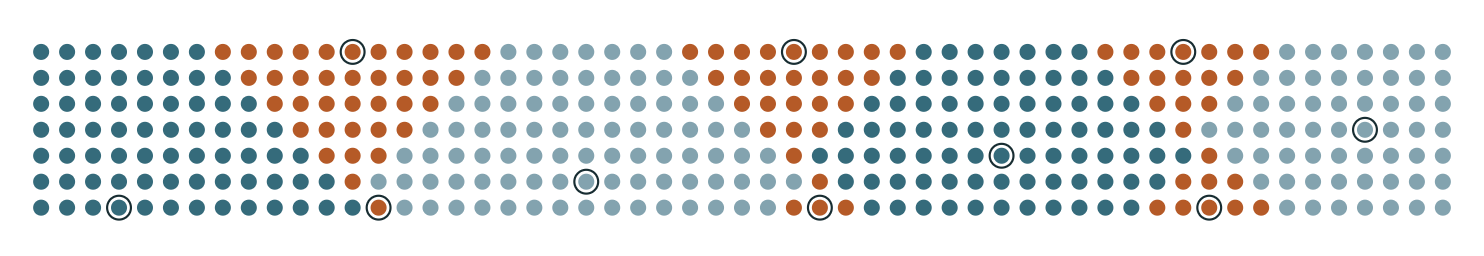
\includegraphics[width=\linewidth]{figure-1.png}
  \caption{七行五十五列网格的十火源覆盖。圆圈标出各火源。}
  \label{fig:fence}
\end{figure}

图 1 中蓝色格点属于四个大球，橙色格点属于六个补缝小球，圆圈标出火源。按实际点火轮次列出的中心与半径如下。最后一列给出在有限矩形内计得的最终球大小。

\begin{center}
\begin{tabular}{rrrrr}
\toprule
轮次 $t$ & $x_t$ & $y_t$ & 半径 $10-t$ & 格点数 \\
\midrule
1 & 3 & 0 & 9 & 70 \\
2 & 21 & 1 & 8 & 87 \\
3 & 37 & 2 & 7 & 79 \\
4 & 51 & 3 & 6 & 58 \\
5 & 12 & 6 & 5 & 36 \\
6 & 29 & 6 & 4 & 25 \\
7 & 44 & 6 & 3 & 16 \\
8 & 45 & 0 & 2 & 9 \\
9 & 30 & 0 & 1 & 4 \\
10 & 13 & 0 & 0 & 1 \\
\bottomrule
\end{tabular}
\end{center}

记第 $t$ 轮的半径为 $\rho_t=10-t$。用 $v=\rho_t-|y-y_t|$ 计算每个球在行 $y$ 的截面；若 $v<0$ 则为空，否则截面为 $[\max(0,x_t-v),\min(54,x_t+v)]\cap\mathbb{Z}$。例如第 $0$ 行按从左至右的次序分成 $[0,12],[13,13],[14,28],[29,31],[32,42],[43,47],[48,54]$，对应火源轮次为 $1,10,2,9,3,8,4$。逐格检查给出七行各 $55$ 个点，每点恰属一个最终球。逐轮同时传播，新增格点数依次为 $1,4,10,19,30,43,57,67,73,81$。九轮若足够，式 \eqref{eq:boundary} 将要求 $55\le9^2-2\cdot3\cdot9+2\cdot3^2=45$，矛盾。因此 $b(7,55)=10$。

随稿的 \texttt{figure-1-sources.csv} 列出十个火源，\texttt{figure-1-rows.csv} 列出七行与十个球的全部 70 个截面（含空截面），\texttt{figure-1-cells.csv} 列出全部 385 个顶点的所属火源与首次燃烧轮次。在源文件目录运行下列命令即可重新核对三份清单，并按行输出各非空区间：

\begin{verbatim}
python verify_figure.py --rows
\end{verbatim}

\section*{参考文献}

[1] Anthony Bonato, Sean English, Bill Kay and Daniel Moghbel. \emph{Improved Bounds for Burning Fence Graphs}. Graphs and Combinatorics \textbf{37} (2021), 2761–2773. \href{https://doi.org/10.1007/s00373-021-02390-x}{期刊版本} · \href{https://arxiv.org/abs/1911.01342}{作者预印本}.
\end{document}